\documentclass[10pt,conference]{IEEEtran}
%\IEEEoverridecommandlockouts
\usepackage[spanish,es-tabla]{babel}
\usepackage[spanish]{babel}
\renewcommand{\baselinestretch}{1.5}     %interlineado
\usepackage[utf8]{inputenc} 
\usepackage[square,numbers]{natbib}
\bibliographystyle{abbrvnat}
\usepackage{float}                      % para usar [H]
\usepackage{amsmath,amssymb,amsfonts}
\usepackage{graphicx}
\usepackage{textcomp}
\usepackage{xcolor}
\usepackage{ragged2e} % \justify

%---------- encabezado pagina
\usepackage{fancyhdr}
\pagestyle{fancy}
\fancyhf{}
\rhead{\thepage}
\renewcommand{\headrulewidth}{0pt}
%-----------------


%-----------------
\def\BibTeX{{\rm B\kern-.05em{\sc i\kern-.025em b}\kern-.08em
    T\kern-.1667em\lower.7ex\hbox{E}\kern-.125emX}}
%__________

\title{Sistemas de Control Difuso \\ {\Large Inteligencia Artificial 2}}
%--------------------------------------------
\author{
\IEEEauthorblockN{1\textsuperscript{do} Angely Mendez}
\IEEEauthorblockA{\textit{Escuela de Informática} \\
\textit{Universidad Nacional de Trujillo}\\
Trujillo, Perú \\
t052701020@unitru.edu.pe}
\and
\IEEEauthorblockN{2\textsuperscript{ero} Ciara Mendez}
\IEEEauthorblockA{\textit{Escuela de Informática} \\
\textit{Universidad Nacional de Trujillo}\\
Trujillo, Perú \\
t022700920@unitru.edu.pe}
}

%%--------------------------------------------
\begin{document}
\renewcommand{\IEEEkeywordsname}{{\bfseries Palabras claves:}} % Colocar Keywords en Spanish

\maketitle
%-------------------------------------------
\begin{abstract}
Este documento es una investigación que describe la Lógica Fuzzy. Este articulo es la recopilación de varias investigaciones a nivel nacional e internacional, en los que abordan un problema y resultados. La Lógica Fuzzy permite resolver un problema en particular después de considerar todos los datos disponibles y luego tomar la decisión adecuada. El método de lógica fuzzy emula la forma humana de tomar decisiones, que considera todas las posibilidades entre valores digitales de Verdadero y Falso y empleados correctamente hacen que un programa exhiba un comportamiento inteligente; respecto a la Lógica Fuzzy, se explica su definición y cuatro investigaciones sobre ella, con la finalidad de entender la importancia de las ciencias de la computación en la vida diaria.  
\end{abstract}

\begin{IEEEkeywords}
Lógica Fuzzy, inferencia difusa, mamdani, TSK, ciencias de la computación, inteligencia artificial.
\end{IEEEkeywords}

\section{\textbf{Introducción}}
Debido a la capacidad insuficiente de las computadoras pequeñas, este enfoque no se aplicó hasta los años 70, donde Lotfi Zadeh, quien introdujo el concepto de Fuzzy Logic (FL) y fue profesor de la Universidad de California en Berkeley, concluyó que las personas no requieren información numérica exacta y, sin embargo, pueden tener un alto control adaptativo.\par 
La lógica fuzzy puede tratar con información que surge de la percepción y la cognición computacionales, es decir, incierta, imprecisa, vaga, parcialmente verdadera o sin límites definidos. La lógica difusa permite la inclusión de evaluaciones humanas vagas en problemas informáticos. Además, proporciona un medio eficaz para la resolución de conflictos de múltiples criterios y una mejor evaluación de las opciones. Los nuevos métodos de computación basados en lógica difusa se pueden utilizar en el desarrollo de sistemas inteligentes para la toma de decisiones, identificación, reconocimiento de patrones, optimización y control. \par 
Entonces este informe presenta información al respecto, el cual está organizado de la siguiente manera: en primer lugar, se explican los conceptos teóricos: definición de la lógica fuzzy y como está conformada, luego se da énfasis en cuatro investigaciones sobre aplicaciones de este tema y para finalizar las conclusiones más relevantes.
%------------------------------------------
\section{\textbf{Lógica Fuzzy}} 
%\vspace{-22 mm}
\subsection{\textbf{\underline{Definición}}}
El término Lógica Difusa fue utilizado por primera vez en 1974. Actualmente se utiliza en un amplio sentido, agrupando la teoría de conjunto difusos, reglas si-entonces, aritmética difusa, cuantificadores, etc. Básicamente la Lógica Difusa es una lógica multivaluada que permite representar matemáticamente la incertidumbre y la vaguedad, proporcionando herramientas formales para su tratamiento.\par
Como indica Zadeh \citep{zadeh1973outline}, “Cuando aumenta la complejidad, los enunciados precisos pierden su significado y los enunciados útiles pierden precisión.”, que puede resumirse como que “los árboles no te dejan ver el bosque”. \par
Básicamente, cualquier problema del mundo puede resolverse como dado un conjunto de variables de entrada (espacio de entrada), obtener un valor adecuado de variables de salida (espacio de salida). La lógica difusa permite establecer este mapeo de una forma adecuada, atendiendo a criterios de significado (y no de precisión). \par
\subsection{\textbf{\underline{Conjuntos Difusos}}}
La lógica multi-valuada, en la definición de grados de pertenencia, la lógica difusa emplea valores contínuos entre 0 (que representa hechos totalmente falsos) y 1 (totalmente ciertos). Así, la lógica binaria clásica puede verse como un caso particular de la lógica difusa. \par
Los conceptos se asocian a conjuntos difusos (asociando los valores de pertenencia) en un proceso llamado \textbf{fuzzificación}. Una vez que tenemos los valores fuzzificados podemos trabajar con reglas lingüísticas y obtener una salida, que podrá seguir siendo \textbf{difusa o defuzzificada} para obtener un valor discreto crisp.\par

\begin{figure}[H]
\begin{center}
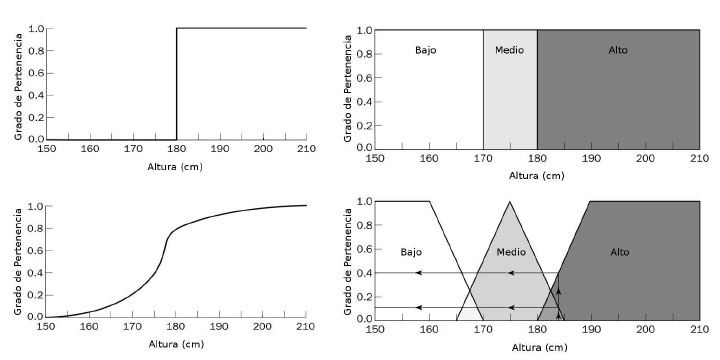
\includegraphics[width=8cm, height=5cm]{figuras/H1.JPG}
\caption{Descripción de conjuntos crisp (arriba) y fuzzy (abajo) de “persona alta”.}
\label{H1} 
\end{center}
\end{figure}

De este modo, a diferencia de la teoría clásica de conjuntos que se basa en el principio básico de la lógica de forma que un individuo pertenece o no pertenece a un conjunto, la idea básica de un conjunto difuso es que un elemento forma parte de un conjunto con un determinado \textbf{grado de pertenencia}.\par
De este modo una proposición no es totalmente (sino parcialmente) cierta o falsa. Este grado se expresa mediante un entero en el intervalo [0, 1].\par


\subsection{\textbf{\underline{Inferencias Difusas}}}
La inferencia difusa puede definirse como el proceso de obtener
un valor de salida para un valor de entrada empleando la teoría de
conjuntos difusos. A continuación veremos dos tipos de inferencia: el
modelo de Mamdani y el de TSK (Takagi, Sugeno y Kang), \citep{gonzalez2015logica}.

\subsubsection{\textbf{\underline{Inferencia de Mamdani}}}
Considerado posiblemente el método más utilizado, propuesto
por Ebrahim Mamdani en 1975. El proceso se realiza en cuatro pasos:
\begin{enumerate}
    \item \textbf{Fuzificación de las variables de entrada:}
    \par
    Toma los valores crisp (cada uno de los componentes de ese vector toma un valor en el conjunto {1,0}) de las entradas y determinar el grado de pertenencia de estas a conjuntos difusos asociados. El valor crisp naturalmente estará limitado en el universo del discurso de la variable.
    \item \textbf{Evaluación de las reglas:}
    \par
    Se toma en cuenta las entradas anteriores y se aplican a los antecedentes de las reglas difusas. Si una regla tiene múltiples antecedentes, utiliza el operador \textbf{AND} u \textbf{OR} para obtener un único número que represente el resultado. Este número (el valor de verdad) se aplica al consecuente.

    \begin{figure}[H]
    \begin{center}
    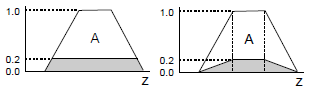
\includegraphics[width=6cm,height=2cm]{figuras/conesca.PNG}
    \caption{Ejemplo gráfico de conjunto recortado y escalado.}
    \label{C1} 
    \end{center}
    \end{figure}

    \item \textbf{Agregación de las salidas de las reglas:}
    \par
    Proceso de unificación de salidas de todas las reglas; mezclan las funciones de pertenencia de consecuentes previamente recortados o escalados, como se muestra en la Figura ~\ref{C1}, obtener un único conjunto difuso por cada variable de salida.
    
    \item \textbf{Defuzificación:} 
    \par
    Se toma como entrada el conjunto difuso anteriormente obtenido para dar un valor de salida. Existen varios métodos de defuzificación, pero probablemente el más ampliamente usado es el \textbf{centroide}. Como se muestra en la Figura ~\ref{C2}.
    
    \begin{figure}[H]
    \begin{center}
    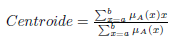
\includegraphics[width=4cm,height=1.3cm]{figuras/ec1.PNG}
    \caption{Fórmula Centroide.}
    \label{C2} 
    \end{center}
    \end{figure}

    Además, según \citep{FuzzyLog14}, el Sistema de Inferencia Difusa, Método Mamdani, en 1975, el profesor Ebrahim Mamdani de la Universidad de Londres construyó uno de los primeros sistemas difusos para controlar una combinación de máquina de vapor y caldera. Aplicó un conjunto de reglas difusas proporcionadas por operadores humanos experimentados, como se muestra en la Figura ~\ref{C3}.
    
    \begin{figure}[H]
    \begin{center}
    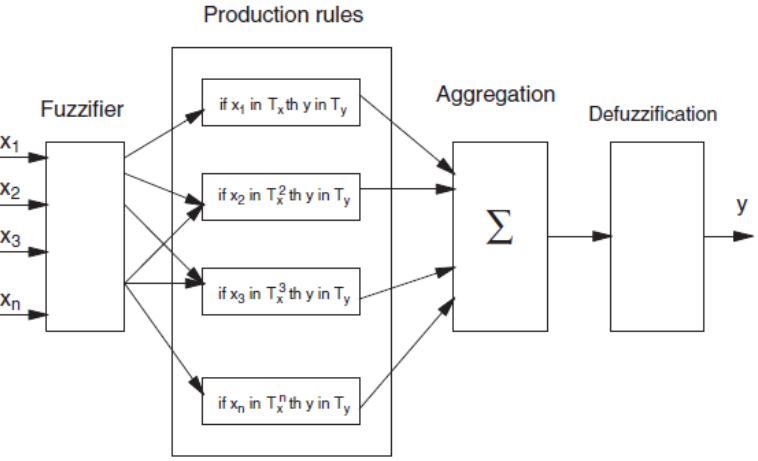
\includegraphics[width=7cm,height=5cm]{figuras/ec2.PNG}
    \caption{Sistema de inferencia borrosa, Fuzzy Inference System.}
    \label{C3} 
    \end{center}
    \end{figure}
\end{enumerate}

\subsubsection{\textbf{\underline{Inferencia de Takagi-Sugeno-Kang (TSK)}}}
En 1985, Takagi y Sugeno aportan a la teoría del control difuso un nuevo método llamado de Takagi-Sugeno-Kang (TSK), como alternativa al método de Mamdani. Se trata de un método basado en reglas difusas pero en el que el consecuente no nos da un conjunto difuso sino una serie de funciones lineales, \citep{diciembre2017sistemas}. Este modelo es útil para sistemas complejos y de dimensiones mayores que los que podemos resolver por el método de Mamdani.

Sean Ai y Bi, con $i$ = $1, 2, ..., n$, conjuntos difusos de nuestro sistema. Las reglas tendrían la forma como en la Figura ~\ref{C36}.

    \begin{figure}[H]
    \begin{center}
    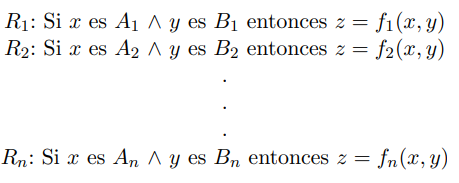
\includegraphics[width=5cm,height=3cm]{figuras/r15.PNG}
    \caption{Forma Reglas TSK.}
    \label{C36} 
    \end{center}
    \end{figure}

La principal diferencia que presenta el método TSK respecto al de Mamdani es que no es necesario realizar un proceso de defuzzificación. Esto se debe al hecho de que no obtenemos ningún conjunto difuso sino un conjunto de funciones lineales. Así, en el método TSK podemos obtener directamente el \textbf{valor de salida de sistema} con una expresión como se muestra en la Figura ~\ref{C35}, \citep{thaker2018analysis}.

    \begin{figure}[H]
    \begin{center}
    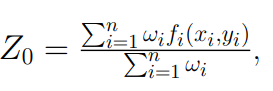
\includegraphics[width=4cm,height=1.5cm]{figuras/ec4.PNG}
    \caption{Media de singletones.}
    \label{C35} 
    \end{center}
    \end{figure}
%-------------------------------------------------------------
A continuación, se presentan cuatro investigaciones donde se evidencia la aplicación de la Lógica Fuzzy:
\begin{enumerate}
\item En la investigación \textit{\textbf{“Sistema de control difuso para riego a tasa variable usando sensores remotos”}}, \citep{MENDES201913}.

\textbf{\underline{Problema:}} 
Evaluando que el riego de tasa variable (VRI) es la capacidad de variar espacialmente la profundidad de la aplicación de agua en un campo para manejar diferentes tipos de suelos, cultivos y otras condiciones. Se deben desarrollar zonas de manejo precisas para aplicar eficientemente las tecnologías de tasa variable. Sin embargo, no existe un método universal para determinar las zonas de gestión. Usar mapas de control de velocidad para el pivote central es una opción. Por lo tanto, esta investigación tiene como objetivo desarrollar un sistema de inferencia borrosa inteligente basado en el conocimiento del riego de precisión (Ver Figura ~\ref{RR1}), un sistema que puede crear mapas prescriptivos para controlar la velocidad de rotación.
    \begin{figure}[H]
    \begin{center}
    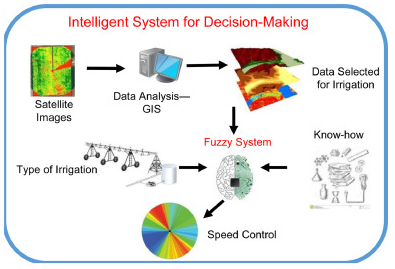
\includegraphics[width=6cm,height=4cm]{figuras/RR1.PNG}
    \caption{Estructura para la estrategia del sistema de riego inteligente.}
    \label{RR1} 
    \end{center}
    \end{figure}
\textbf{\underline{Resultados:}} 
El sistema de riego inteligente señaló zonas con menor desarrollo foliar, indicando que el pivote debe reducir su velocidad, aumentando así la capa de agua aplicada en la zona. La consigna construida por el sistema desarrollado señalaba zonas con una disminución de velocidad del orden del 50\%. El sistema propuesto obtuvo valores de 37\% y 47\% para ajustar el temporizador de porcentaje de pivote. Los resultados indican que los datos de las variables edafoclimáticas, cuando se ajustan bien a la lógica difusa, ver Figuras ~\ref{RR2} y ~\ref{RR22}, pueden resolver las incertidumbres y no linealidades de un sistema de riego y establecer un modelo de control para el riego de alta precisión, ver Figura ~\ref{RR3}. Donde dentro del objetivo propuesto para el sistema desarrollado, una vez aplicadas las variables lingüísticas a la salida de los sistemas de inferencia borrosa, se vuelve más apto para modelar el proceso de reflexión humana. Al hacerlo, la interfaz del sistema se vuelve más sencilla y natural. Además, las salidas difusas, que representan la velocidad de rotación del pivote central, se construyeron a partir de cinco variables lingüísticas: muy baja (MB), baja (B), normal (N), alta (A) y muy alta (MA). Todos los conjuntos se interpretaron en función de sus funciones de pertenencia, como se muestra en la Fig. ~\ref{RR33} . Y el método de defuzzificación utilizado fue CENTROID (centro de área o centro de gravedad). 

    \begin{figure}[H]
    \begin{center}
    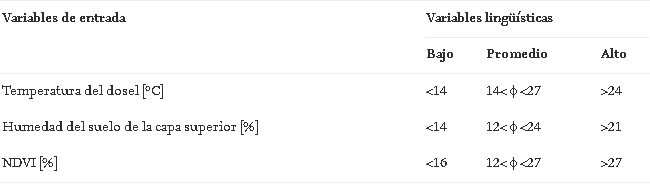
\includegraphics[width=7cm,height=2cm]{figuras/RR2.PNG}
    \caption{Reglas difusas para el control de la velocidad del pivote central.}
    \label{RR2} 
    \end{center}
    \end{figure}
    
    \begin{figure}[H]
    \begin{center}
    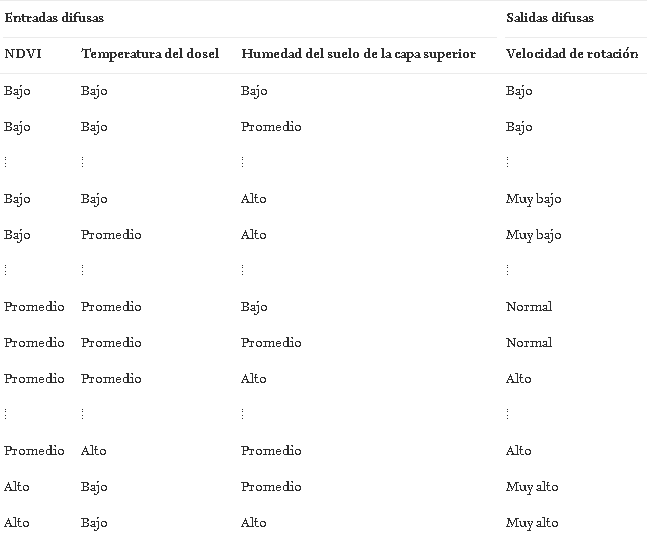
\includegraphics[width=8cm,height=3.5cm]{figuras/RR22.PNG}
    \caption{Reglas difusas para el control de la velocidad del pivote central.}
    \label{RR22} 
    \end{center}
    \end{figure}
    
    \begin{figure}[H]
    \begin{center}
    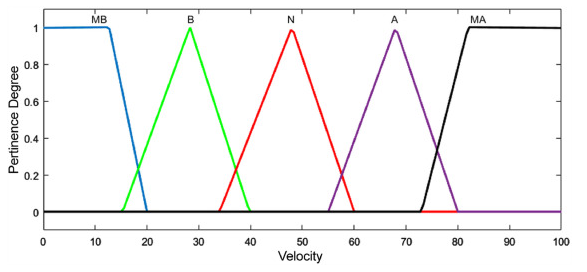
\includegraphics[width=7cm,height=3cm]{figuras/RR3.PNG}
    \caption{Funciones de pertenencia correspondientes a cada entrada del sistema.}
    \label{RR3} 
    \end{center}
    \end{figure}
    
    \begin{figure}[H]
    \begin{center}
    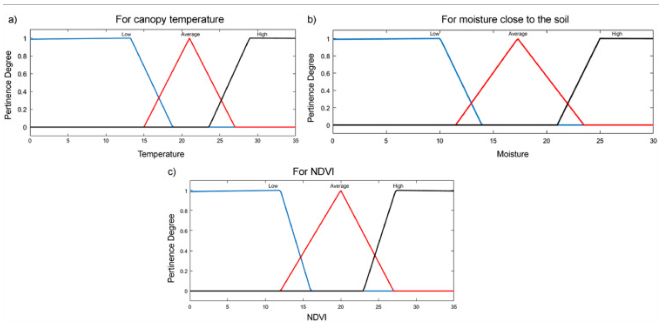
\includegraphics[width=8cm,height=5cm]{figuras/RR33.PNG}
    \caption{Funciones de pertenencia para la velocidad correspondiente a la etapa de defuzzificación.}
    \label{RR33} 
    \end{center}
    \end{figure}
    
\textbf{\underline{Importancia:}} 
El sistema fuzzy desarrollado para el control del riego es original e innovador. En ese contexto, la lógica difusa se puede aplicar ampliamente en áreas agrícolas; por lo tanto, es beneficioso porque puede construir un sistema de apoyo a la decisión que tenga el conocimiento del riego de precisión. Y la implementación del sistema de soporte de decisiones de lógica difusa fue útil y exitosa para desarrollar mapas de prescripción para VRI con pivotes centrales, debido a que, el modelo de lógica difusa funcionó como se esperaba, brindando excelentes resultados.

\item Otra investigación \textit{\textbf{“Diseño de un sistema de control difuso para la estabilidad de los niveles de las celdas de flotación en un proceso continuo cuprífero”}}, \citep{haro2019diseno}.

\textbf{\underline{Problema:}} 
La evolución de la minería a lo largo de los años ha permitido el desarrollo de nuevas
técnicas de procesamiento, el siglo XXI con un aporte importante de la ingeniería de control, de mejorar los indicadores de productividad y calidad. En la etapa de flotación, se añade a la pulpa los reactivos idóneos en proporciones
adecuadas. Debido a la variabilidad del mineral y los métodos de acondicionamiento vigentes, la etapa de flotación trata y reutiliza al máximo la pulpa. Esta investigación considera que el problema se debe a que el sistema de recuperación en todas las celdas se encuentran conectadas propagando la
inestabilidad en todo el ciclo, por lo que tiene como objetivo diseñar y simular un sistema de control difuso para mantener la estabilidad de los niveles
de las celdas de flotación en un proceso continuo cuprífero, ver Figura ~\ref{AA1}.

    \begin{figure}[H]
    \begin{center}
    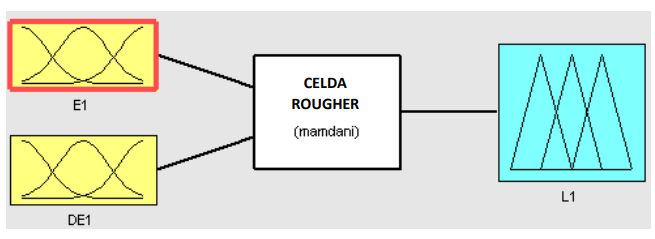
\includegraphics[width=8cm,height=3cm]{figuras/AA1.PNG}
    \caption{Configuración del controlador difuso para celda Scavenger.}
    \label{AA1} 
    \end{center}
    \end{figure}

\textbf{\underline{Resultados:}} 
Con el diseño del controlador difuso de tipo directo con retroalimentación se
demostró la exigencia del conocimiento del comportamiento de la variable de
control y experiencia del usuario en el proceso, para la definición de las variables
difusas (Ver Figuras ~\ref{AA2}, ~\ref{AA3} y ~\ref{AA4}), funciones de membresía y reglas difusas (ver Figuras ~\ref{AA5} ), con ello, la obtención de una respuesta flexible frente a un sistema complejo de control directo e inverso simultáneamente, imposible desde un punto de vista de control clásico.

    \begin{figure}[H]
    \begin{center}
    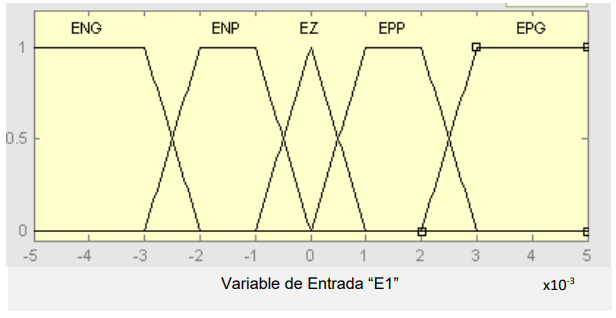
\includegraphics[width=8cm,height=2.5cm]{figuras/AA2.PNG}
    \caption{Gráfico de las funciones de membresía de la variable difusa E1.}
    \label{AA2} 
    \end{center}
    \end{figure}

     \begin{figure}[H]
    \begin{center}
    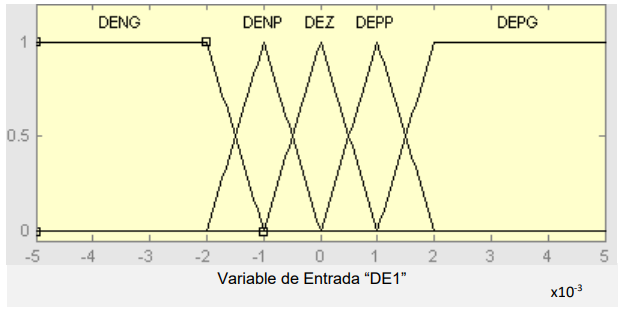
\includegraphics[width=8cm,height=2.5cm]{figuras/AA3.PNG}
    \caption{Gráfico de las funciones de membresía de la variable difusa DE1.}
    \label{AA3} 
    \end{center}
    \end{figure}

     \begin{figure}[H]
    \begin{center}
    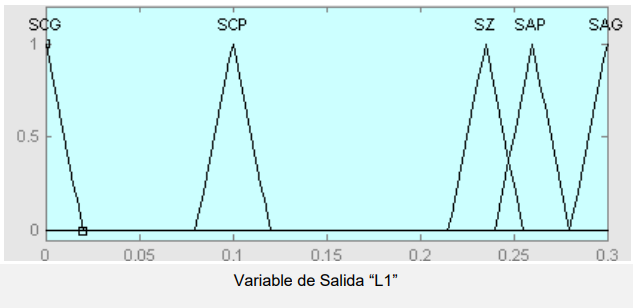
\includegraphics[width=8cm,height=2.5cm]{figuras/AA4.PNG}
    \caption{Gráfico de las funciones de membresía de la variable difusa L1.}
    \label{AA4} 
    \end{center}
    \end{figure}

    \begin{figure}[H]
    \begin{center}
    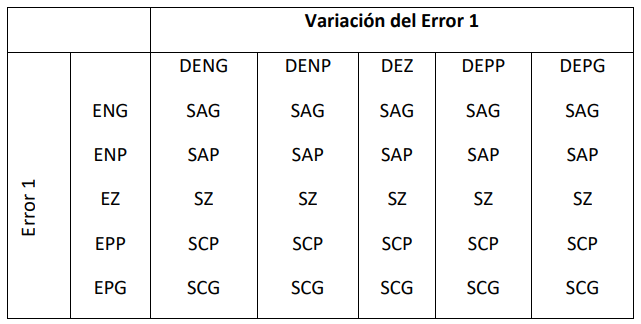
\includegraphics[width=8cm,height=2.5cm]{figuras/AA5.PNG}
    \caption{Reglas difusas para controlador.}
    \label{AA5} 
    \end{center}
    \end{figure}


    
La integración de los softwares industriales de Rockwell Automation y National
Instruments fueron satisfactorios y eficientes para simular el modelo matemático
diseñado con un tiempo de muestreo seteado a 50 ms. En la simulación con el
controlador proporcional integrativo, el tiempo de muestreo se mantuvo en el rango
de 46 ms a 297 ms, a diferencia de la simulación con el controlador difuso que se
mantuvo entre 46 ms a 63 ms.

\textbf{\underline{Importancia:}} 
La implementación del control difuso benefician directamente a Tecsup o
una unidad minera interesada por el ahorro económico en producción y mantenimiento que
conlleva, y beneficios indirectos como reducción del concentrado del relave emitido al
ambiente. Además, el comportamiento del proceso con el controlador difuso directo propuesto, fue adecuado y se midió el tiempo de arranque cuando todos los niveles de las celdas alcanzaron el valor de consigna. 

%-----------------------------------------------------------------
\item En la investigación \textit{\textbf{“Un supervisor de lógica difusa para el control PID de sistemas desconocidos”}}, \citep{copeland1994fuzzy}.\par
\textbf{\underline{Problema:}}
Debido a la falta de sistemas para reducir la cantidad de sintonización, se plantea el diseño de un supervisor de lógica difusa para controladores de DP diseñados utilizando las reglas de sintonía de Ziegler-Nichols. Dado que Ziegler-Nichols proporciona valores de parámetros nominales para el controlador de PD, la respuesta deseada del sistema no puede lograrse sin un ajuste adicional del controlador. Este supervisor difuso permite reducir la cantidad de ajustes adicionales. El objetivo del supervisor difuso es aumentar gradualmente las ganancias proporcional y derivativa del controlador, a medida que el error del sistema se acerca a cero, para mejorar la respuesta del sistema. 
    \begin{figure}[H]
    \begin{center}
    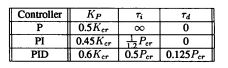
\includegraphics[width=5cm,height=1.5cm]{figuras/N1.JPG}
    \caption{Reglas de ajuste de Ziegler-Nichols basadas en la ganancia crítica y el período de oscilación.}
    \label{N1} 
    \end{center}
    \end{figure}

    \begin{figure}[H]
    \begin{center}
    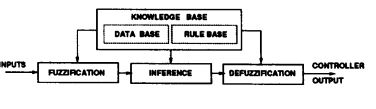
\includegraphics[width=6cm,height=2cm]{figuras/N2.JPG}
    \caption{: Controlador de lógica difusa.}
    \label{N2} 
    \end{center}
    \end{figure}

\textbf{\underline{Resultados:}}
Se demuestra que el rendimiento de los sistemas controlados por controladores PD (diseñados con las reglas de ajuste de Ziegler-Nichols) mejora con la adición del supervisor de lógica difusa (FLS). También se demuestra (mediante simulación) que un aumento gradual en la ganancia proporcional (KP) del controlador, a medida que disminuye el error del sistema, da como resultado una respuesta mejorada del sistema. La ganancia derivada (KD) se determina inicialmente multiplicando la nueva ganancia proporcional por la relación de los parámetros originales (KDKP). Luego, cuando el error del sistema se aproxima a cero, la ganancia derivada aumenta para eliminar las oscilaciones debidas al aumento del valor de KP.(Ver Figuras ~\ref{N3}, ~\ref{N4} y ~\ref{N5})

    \begin{figure}[H]
    \begin{center}
    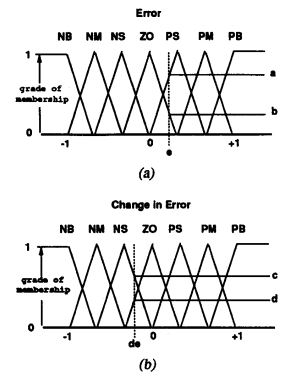
\includegraphics[width=5.5cm,height=4cm]{figuras/N3.JPG}
    \caption{Funciones de pertenencia triangulares.}
    \label{N3} 
    \end{center}
    \end{figure}

    \begin{figure}[H]
    \begin{center}
    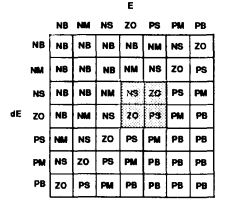
\includegraphics[width=6cm,height=3cm]{figuras/N4.JPG}
    \caption{Matriz de reglas difusas de Macvicar-Whelm.}
    \label{N4} 
    \end{center}
    \end{figure}

    \begin{figure}[H]
    \begin{center}
    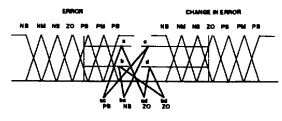
\includegraphics[width=8cm,height=3cm]{figuras/N5.JPG}
    \caption{Generación de salida difusa.}
    \label{N5} 
    \end{center}
    \end{figure}

\textbf{\underline{Importancia:}} 
Las reglas de ajuste de Ziegler-Nichols se desarrollaron para ayudar en el diseño de controladores para sistemas desconocidos; sin embargo, las técnicas también se pueden aplicar a sistemas con funciones de transferencia conocidas. Para demostrar el efecto del supervisor difuso, se implementó el método de Ziegler-Nichols en dos sistemas con funciones de transferencia conocidas. El primer sistema (un sistema de tipo 0) es un brazo flexible de enlace único y el segundo ejemplo (un sistema de tipo 1) es un sistema de servomotor.
%-----------------------------------------------------------------
\item Otra investigación \textit{\textbf{“Sistema de Control Automático de Nivel de Agua en la Cámara de Carga Basado en la Lógica Difusa para la Central Hidroeléctrica de Machupicchu”}}, \citep{meza2019sistema}.\par
\textbf{\underline{Problema:}} 
La Empresa de Generación Eléctrica Machupicchu S.A. (EGEMSA) es una empresa dedicada a la
generación y comercialización de energía eléctricas. Las primeras edificaciones se hicieron en los años 60 y 80, sin embargo,
en el año 1998, el deslizamiento que ocurrió en la quebrada Aobamba, dejó sepultada a la central. Cuando el nivel de agua es muy bajo, existe la posibilidad de ingreso de aire a la tubería forzada que ocasionaría pulsaciones y oscilaciones de presión en el circuito hidráulico; es decir, principalmente, dañarían a los equipos asociados a la turbina Francis. Las variaciones pronunciadas de nivel de agua en la cámara de carga sumado con la regulación por métodos tradicionales, pone en riesgo a la operación eficiente de la turbina Francis y a los equipos asociados en la Central Hidroeléctrica de Machupicchu.(Ver Figuras ~\ref{M1} y ~\ref{M2})

    \begin{figure}[H]
    \begin{center}
    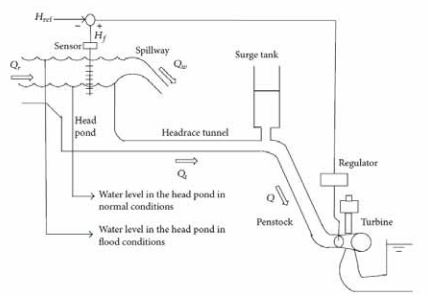
\includegraphics[width=6cm,height=4cm]{figuras/M1.JPG}
    \caption{Central hidroeléctrica típica de desviación del curso del río.}
    \label{M1} 
    \end{center}
    \end{figure}

     \begin{figure}[H]
    \begin{center}
    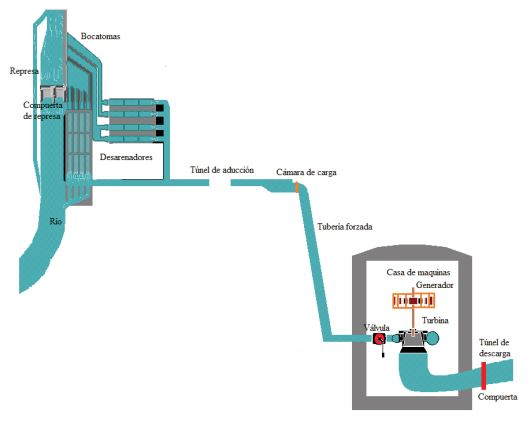
\includegraphics[width=7cm,height=5cm]{figuras/M2.JPG}
    \caption{Partes de una central hidroeléctrica de pasada de río.}
    \label{M2} 
    \end{center}
    \end{figure}

\textbf{\underline{Resultados:}} 
Se diseñó un sistema de control difuso con dos entradas (error y pendiente de nivel de agua) y una salida (variación de carga de la turbina Pelton) utilizando el método general que planteó Ebrahim H. Mamdani para automatizar sistemas no lineales; la data fundamental para el diseño fue el registro de datos de nivel de agua para la determinación de las funciones de pertenencia de entradas y salida del controlador difuso y el conocimiento de operación de experto en la regulación de nivel de agua en la cámara de carga. En las pruebas finales, con la sintonización apropiada con 27 reglas de inferencia difusa y con los siguientes parámetros del controlador difuso: Kp=1, Kd=100, Ku=1, se logró mantener el nivel de agua en la cámara de carga dentro del margen requerido con un error ±0.20 m con respecto a la referencia del nivel de agua.(Ver Figuras ~\ref{M3}, ~\ref{M4} y ~\ref{M5})

    \begin{figure}[H]
    \begin{center}
    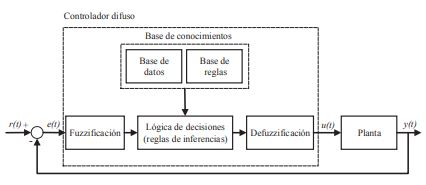
\includegraphics[width=6cm,height=4cm]{figuras/M3.JPG}
    \caption{ Sistema de control difuso realimentado.}
    \label{M3} 
    \end{center}
    \end{figure}

     \begin{figure}[H]
    \begin{center}
    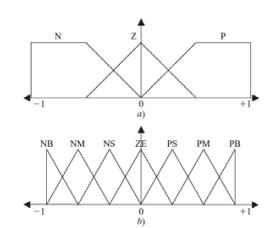
\includegraphics[width=6cm,height=4cm]{figuras/M4.JPG}
    \caption{Generación de valores difusos.}
    \label{M4} 
    \end{center}
    \end{figure}

    \begin{figure}[H]
    \begin{center}
    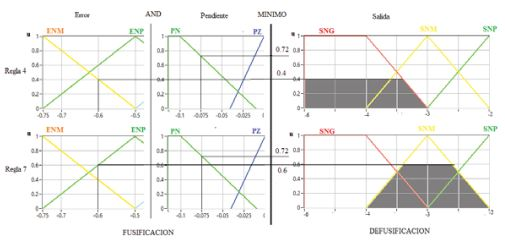
\includegraphics[width=8cm,height=4cm]{figuras/M5.JPG}
    \caption{Interpretación gráfica del proceso de defuzzificación.}
    \label{M5} 
    \end{center}
    \end{figure}

\textbf{\underline{Importancia:}} 
El controlador difuso implementado en la plataforma de desarrollo LabVIEW, en un computador de escritorio; obtiene el dato de entrada, medición de nivel de agua de la cámara de carga, por medio de conexión cliente OPC del sistema SCADA de la planta. El algoritmo de control basado en lógica difusa de tipo PD (proporcional-derivativo), implementado usando la herramienta “Fuzzy Logic Control”, determina la variación de carga de la turbina; posteriormente este valor es enviado al PLC principal de uno de los generadores Pelton, a través de otro servidor OPC sobre la red Ethernet.


\end{enumerate} 
%------------------------------------------------------------------
\section{\textbf{Conclusiones}}
Este informe presentó información relevante acerca de Lógica Fuzzy empleadas en la Inteligencia Artificial, explicándose también los conceptos teóricos relacionados a ella. Además de permitir conocer sobre algunas investigaciones que se vienen realizando año a año, entendiendo las diversas aplicaciones en diversos campos de la vida diaria. Concluimos que la mayoría analiza la problemática y dependiendo de sus características se estableció las variables, reglas difusas y método de defuzificación para representar o modelar la información y el sistema de control o software a emplear. Finalmente, las investigaciones expuestas en este trabajo de recopilación, sirven como antecedentes y base a futuros investigadores a nivel nacional e internacional, que pueden ser usados tanto en el área comercial o académico.
%-------------------------------------------------------
\medskip
\bibliography{refer}
\end{document}